\chapter{Related Work}
\label{chap:RelatedWork}


\section{CVC-MUSCIMA Dataset}
\label{sec:CvcMuscima}

CVC-MUSCIMA is a~dataset presented in the article: \emph{CVC-MUSCIMA: A ground truth of handwritten music score images for writer identification and staff removal} (\cite{CvcMuscima}). This dataset contains 1000~sheets of~music, consisting of 20~pages, each written by 50~different musicians. It's the~only publicly available dataset containing entire staves of handwritten music. The~dataset has been designed for writer identification and staff (staff line) removal tasks. It contains two sets of images. One set for writer identification (containing gray, binary, and staff-less binary images) and one set for staff removal (contains raw, staff-less, and staff-only images, all binary).

\begin{figure}[h]
    \centering
    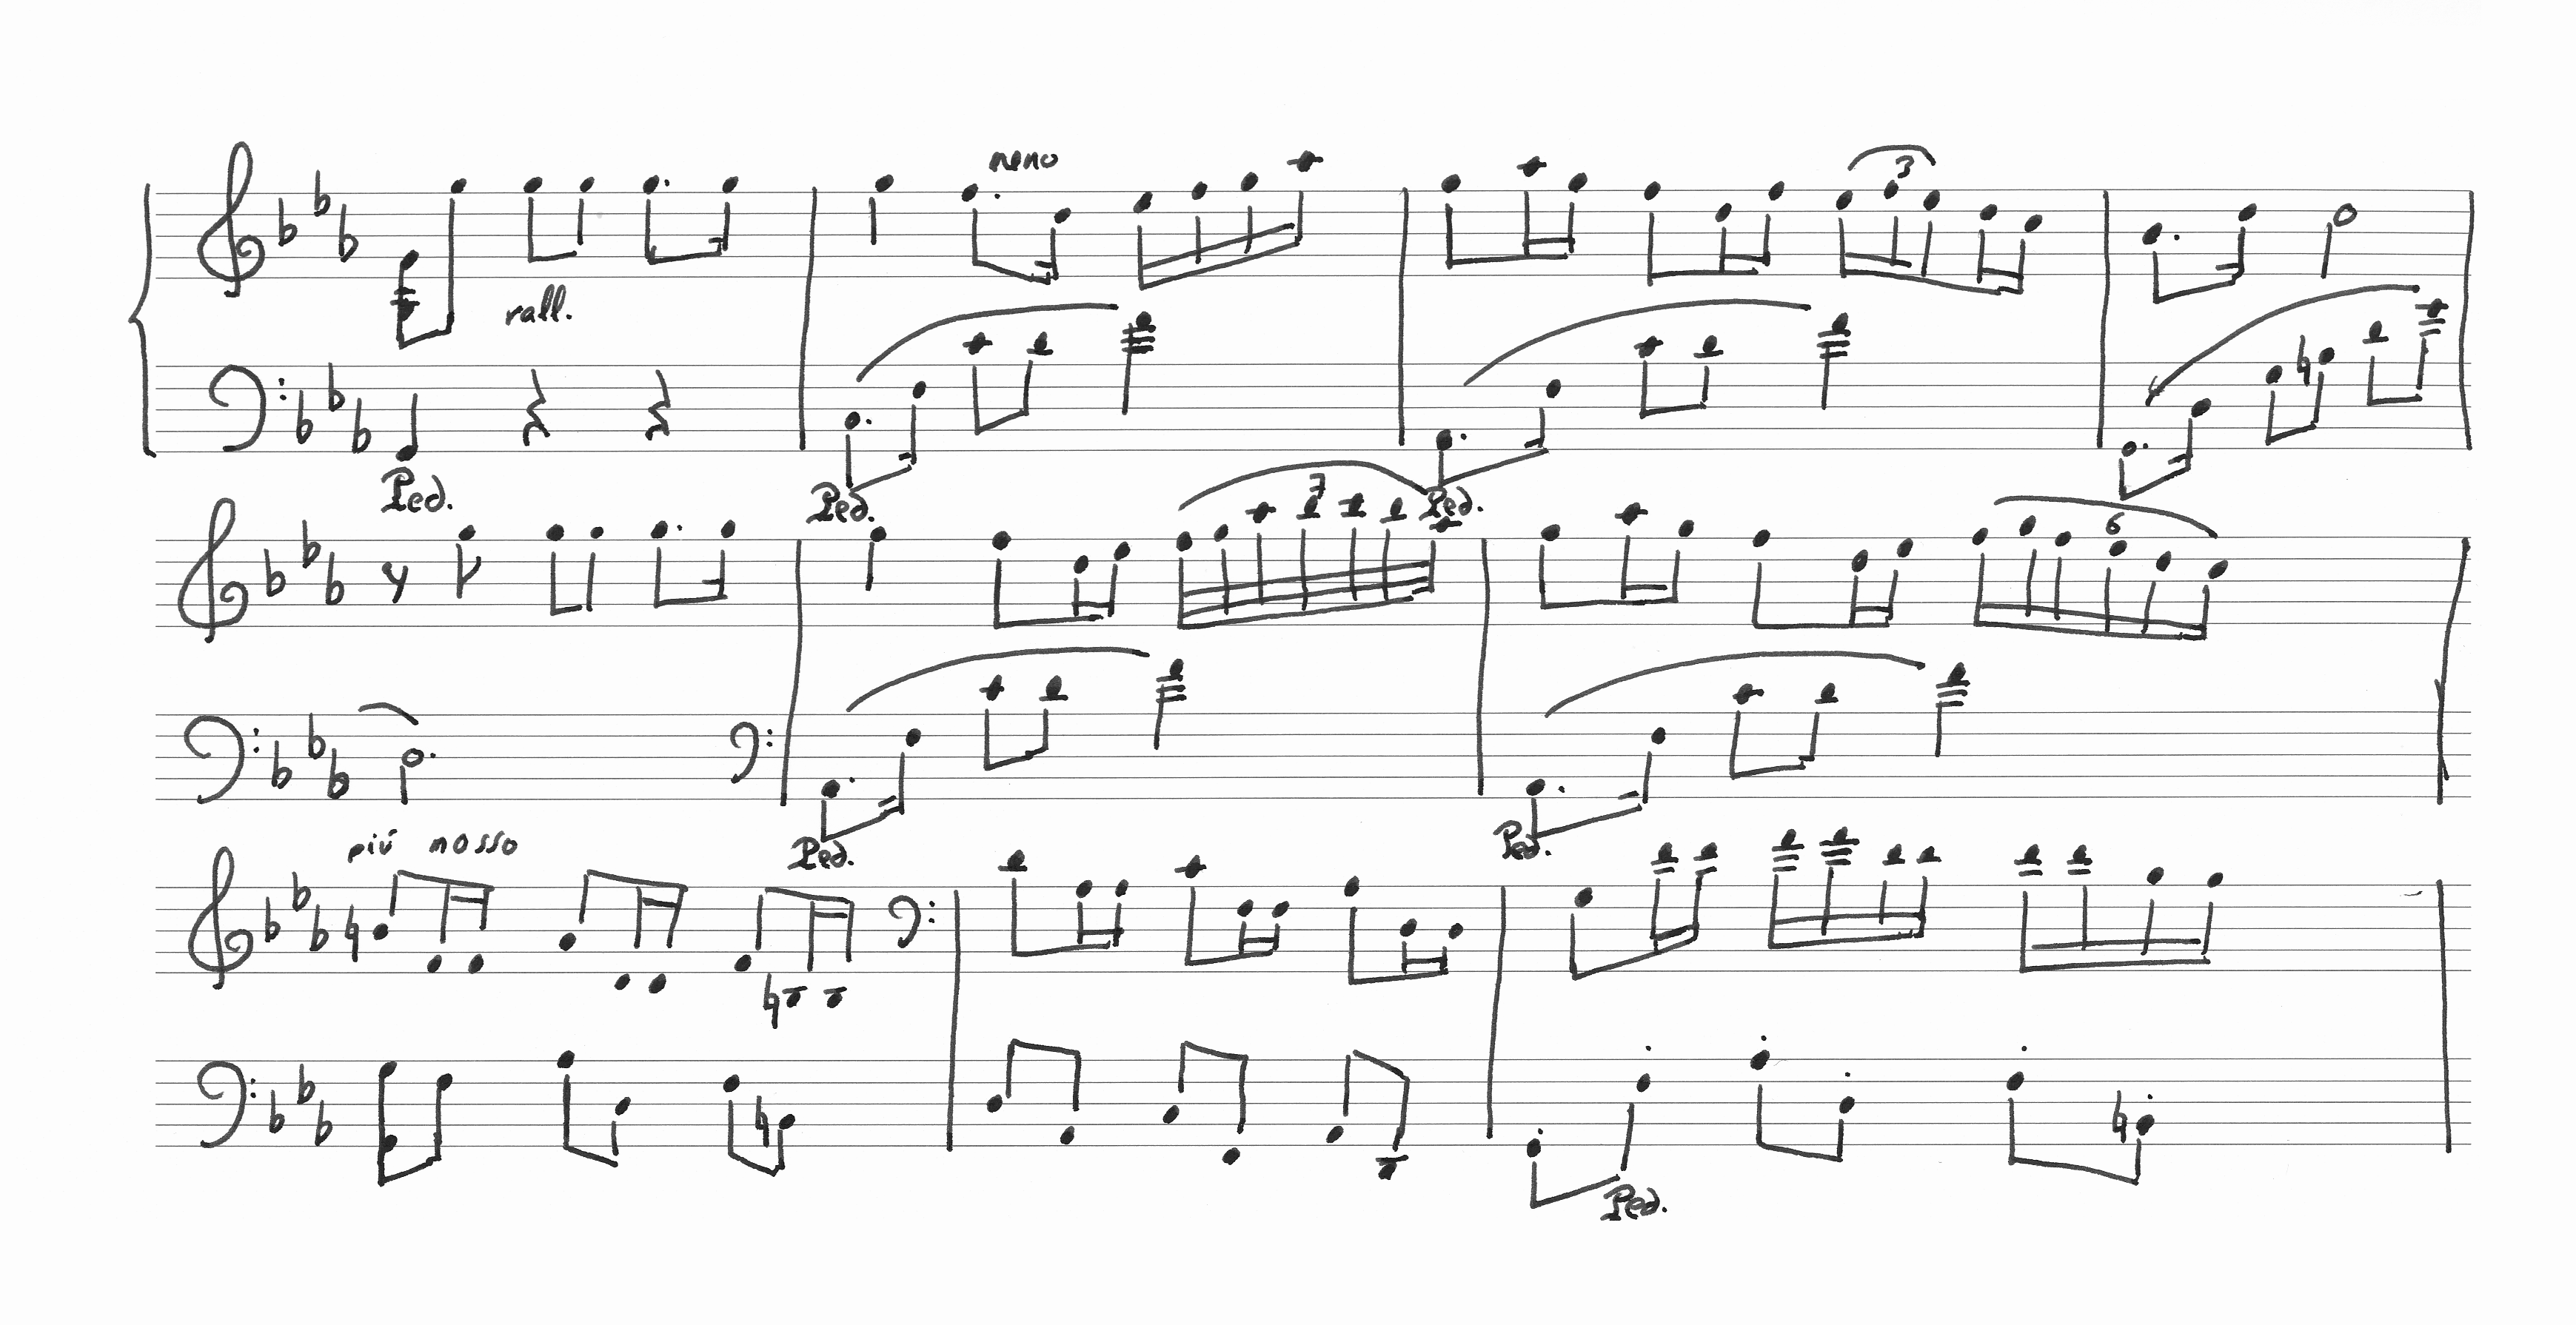
\includegraphics[width=140mm]{../img/cvc-muscima}
    \caption{One sheet of music from the CVC-MUSCIMA dataset. Image taken from the CVC-MUSCIMA website \href{http://www.cvc.uab.es/cvcmuscima/index_database.html}{\texttt{http://www.cvc.uab.es/{\allowbreak}cvc{\allowbreak}muscima/{\allowbreak}index\_database.html}}.}
    \label{fig2:CvcMuscima}
\end{figure}

We will use part of the~staff removal set for evaluation. We will also use another part of the~staff removal set for engraving, but indirectly via the MUSCIMA++ dataset.


\section{MUSCIMA++ Dataset}

MUSCIMA++ is a~dataset developed by Jan Hajič~jr. and Pavel Pecina and has been presented in the~article: \emph{In Search of a Dataset for Handwritten Optical Music Recognition: Introducing MUSCIMA++} (\cite{MuscimaPP}). This dataset provides additional information for a~subset of the~CVC-MUSCIMA dataset. MUSCIMA++ contains 140~sheets of music. Each sheet is annotated at the~level of individual symbols (noteheads, stems, flags, beams, slurs, staff lines). Each one of these symbols is classified, contains a~bounding box and a~pixel mask. These symbols are then interlinked in a~graph that can be traversed to extract higher-level objects (notes, key signatures, beamed note groups).

\begin{figure}[h]
    \centering
    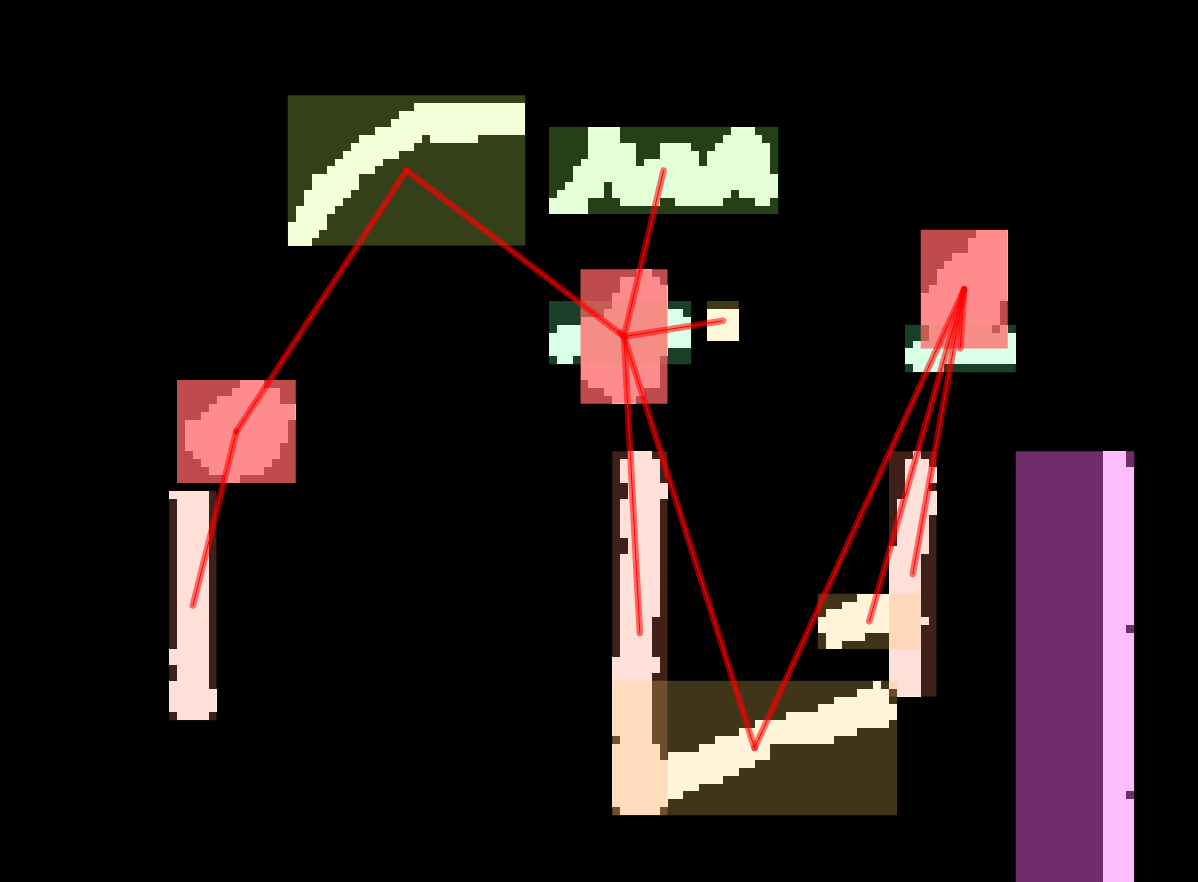
\includegraphics[width=100mm]{../img/muscima-pp}
    \caption{Notation graph of the MUSCIMA++ dataset. Image taken from \cite{MuscimaPP}.}
    \label{fig2:MuscimaPP}
\end{figure}

We will use the~dataset as a~collection of musical symbols. We will then place those symbols onto an~empty staff to create synthetic training data. The additional data (relationship graph) will help us position certain symbols properly.


\section{End-to-End OMR and the PrIMuS Dataset}

This section refers to the~article: \emph{End-to-End Neural Optical Music Recognition of Monophonic Scores} (\cite{Primus}). This article first describes the~PrIMuS\footnote{\href{https://grfia.dlsi.ua.es/primus/}{https://grfia.dlsi.ua.es/primus/}} dataset. This dataset contains 87678~real-music incipits. An~incipit is the~part of a~melody or a~musical work that is most recognizable for that work. Each incipit is a~few measures long, typically shorter than a~single staff of printed sheet music. Each incipit is encoded in a~few widely known encodings (MEI, MIDI) and has a corresponding printed image. This image has been engraved using the~music notation engraving library Verovio\footnote{\href{https://www.verovio.org/}{https://www.verovio.org/}}. Each incipit is also encoded using two on-purpose devised encodings --- the PrIMuS semantic and agnostic encoding. These encodings are interesting because they are the~output of a~model proposed in the~article, but also the~Mashcima encoding described in chapter \ref{chap:MusicRepresentation} of this thesis is very similar to the~agnostic encoding.

\begin{figure}[h]
    \centering
    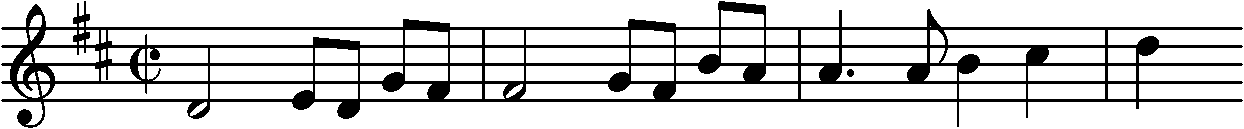
\includegraphics[width=120mm]{../img/primus-incipit}
    \\
    \medskip
    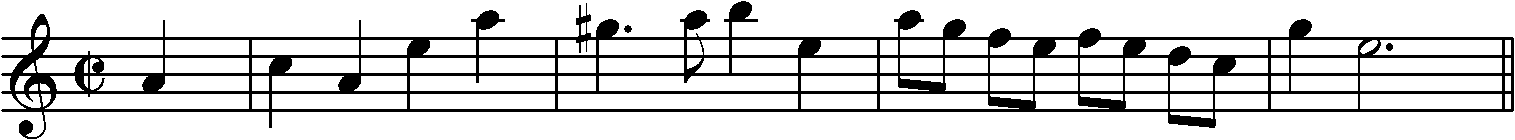
\includegraphics[width=140mm]{../img/primus-incipit-2}
    \caption{Two incipits taken directly from the PrIMuS dataset.}
    \label{fig2:PrimusIncipits}
\end{figure}

The~article also proposes a~neural network architecture for an~end-to-end solution of~OMR. The~architecture is very similar to ours, almost identical. It also uses the~connectionist temporal classification as the loss function (\cite{CTC}), which shapes the~PrIMuS dataset encoding formats. This thesis differs from this article mainly in the~focus on~handwritten music and the~introduction of~a~custom engraving system for handwritten music. The PrIMuS article focuses on~printed music only.

We will use the~PrIMuS dataset as a~source of~melodies that can be used as~input to~our engraving system. We will also take this article as~a~basis for our Mashcima encoding and our model architecture.


\section{HMR Baseline Article}

This section refers to the~article: \emph{From Optical Music Recognition to Handwritten Music Recognition: A baseline} (\cite{HmrBaseline}). This paper proposes a~model that should serve as a~baseline for handwritten music recognition. The model is again a~convolutional recurrent neural network that recognizes entire staves. The model is trained on~printed music and then, using transfer learning, fine-tuned on handwritten music. The handwritten music comes from the~MUSCIMA++ dataset and it has been varied using data augmentation (blurring, erosion, dilation, measure shuffling). This model, however, does not use the CTC loss function, instead, it produces two vectors for each pixel of the~input image width. One vector contains symbols that are present in the~image at~that position and the~other vector contains pitches of~these symbols. This means annotations have to be aligned with the symbols (unlike with CTC), but it allows the~model to recognize dense music sheets and even chords.

We will attempt to compare our model to the~one from this article. The~comparison will be difficult because the~output formats are so~different, but we will mention all the~differences and add a~qualitative comparison of the~final predictions. We want to utilize the fact that our evaluation dataset intersects with theirs and~so we can perform a~direct comparison.
